\chapter{Технологический раздел}
В технологическом разделе выбраны и описаны средства реализации программного обеспечения и представлены детали его реализации.

Для реализации программного обеспечения был выбран язык программирования $Rust$~\cite{rust2024}, так как он позволяет реализовать все алгоритмы, выбранные в результате проектирования и поддерживает все требуемые структуры данных.

Был выбран фреймворк $egui$~\cite{egui2024} для реализации интерфейса программного обеспечения, так как в нём присутствуют инструменты для работы с изображениями и разработки интерфейса.

\section{Реализация алгоритмов}

В листинге~\ref{lst:visit-cloud} представлен листинг функции отрисовки облака.
\begin{lstlisting}[style=rust, caption={Фунция отрисовки облака},label={lst:visit-cloud}]
fn visit_cloud(&mut self, cloud: &Cloud) {
	use rayon::prelude::*;
	
	let bb = cloud.bounding_box();
	
	let (w, h) = self.canvas.size();
	let light_color: Vec4 = cloud.light_color.into();
	let sun_pos = sun.map(|x| x.get_pos()).unwrap_or_default();
	let ray_origin = self.camera.pos();
	img.pixels.par_iter_mut().enumerate().for_each(|(idx, pixel)| {
		let i = idx / w + min_tuple.y as usize;
		let j = idx % w + min_tuple.x as usize;
		
		let ray_dir = (self.camera.egui_to_world(i, j, w, h) - ray_origin).normalize();
		let ray_box_info = bb.dst(ray_origin, ray_dir);
		let dst_to_box = ray_box_info.x;
		let dst_inside_box = ray_box_info.y;
		
		if dst_inside_box <= 0.0 {
			*pixel = Color32::TRANSPARENT
		} else {
			let mut dst_travelled = 0.0;
			let dst_limit = dst_inside_box;
			let step_size = dst_inside_box / cloud.num_steps as f32;
			let mut transmittance = 1.0;
			let mut light_energy = 0.0;
			
			let entry_point = ray_origin + dst_to_box * ray_dir;
			let cos_angle = ray_dir.dot(sun_pos);
			let phase = phase(cos_angle.abs(), cloud.phase_params);
			
			while dst_travelled < dst_limit {
				let ray_pos = entry_point + ray_dir * dst_travelled;
				let density = cloud.sample_density(ray_pos);
				if density > 0.1 {
					let light_transmittance = cloud.light_march(ray_pos, sun_pos);
					light_energy +=
					density * step_size * transmittance * light_transmittance * phase;
					transmittance *=
					beer(density * step_size * cloud.light_absorption_through_cloud);
					if transmittance < 0.01 {
						break;
					}
				}
				dst_travelled += step_size;
			}
			
			*pixel = if transmittance >= 0.01 {
				Color32::TRANSPARENT
			} else {
				let focused_eye_cos = cos_angle
				.clamp(-std::f32::consts::PI, std::f32::consts::PI)
				.powf(cloud.params.x);
				let sun = hg(focused_eye_cos, 0.995).clamp(-1.0, 1.0) * transmittance;
				
				let cloud_col = light_energy * light_color.xyz();
				let col = cloud_col.clamp(Vec3::ZERO, Vec3::ONE) * (1.0 - sun)
				+ light_color.xyz() * sun;
				let (r, g, b) = col.into();
				Color32::from_rgb(
				(r * 255.0) as u8,
				(g * 255.0) as u8,
				(b * 255.0) as u8)
			};
		}
	});
}
\end{lstlisting}
\newpage
В листинге~\ref{lst:light-march} представлен листинг функции определения затухания света от солнца в точке облака.
\begin{lstlisting}[style=rust, caption={Определение затухания света от солнца в точке облака.},label={lst:light-march}]
pub fn light_march(&self, mut p: Vec3, world_space_light_pos0: Vec3) -> f32 {
	let dir_to_light = world_space_light_pos0;
	let dst_inside_box = self.bounding_box().dst(p, dir_to_light).y;
	let step_size = dst_inside_box / self.num_steps_light as f32;
	p += dir_to_light * step_size;
	
	let mut total_density = 0.0;
	let step_size_f32 = step_size;
	
	for _ in 0..self.num_steps_light {
		let density = self.sample_density(p);
		total_density += density.max(0.0) * step_size_f32;
		p += dir_to_light * step_size_f32;
	}
	
	let transmittance = beer(total_density * self.light_absorption_toward_sun);
	transmittance.lerp(1.0, self.darkness_threshold)
}
\end{lstlisting}

В листинге~\ref{lst:generate-grid}  представлен листинг функции генерации ландшафтной сетки.
\begin{lstlisting}[style=rust, caption={Функция генерации ландшафтной сетки.},label={lst:generate-grid}]
	pub fn generate_grid(&mut self) {
		use rayon::prelude::*;
		let bb = self.bounding_box;
		let min = bb.min;
		let max = bb.max;
		let scale = self.scale;
		
		let sample_y = self.noise_weight.x;
		let sample_z = self.noise_weight.y;
		let noise = &self.perlin;
		
		let vec: Vec<_> = (0..self.scale)
		.into_par_iter()
		.flat_map(|z| {
			(0..=self.scale)
			.into_par_iter()
			.map(move |x| {
				let x_frac = x as f32 / scale as f32;
				let z_frac = z as f32 / scale as f32;
				let next_z_frac = (z + 1) as f32 / scale as f32;
				
				let base_x = min.x + (max.x - min.x) * x_frac;
				let base_z = min.z + (max.z - min.z) * z_frac;
				let next_z = min.z + (max.z - min.z) * next_z_frac;
				
				let sample_pos = bb.min
				+ Vec3::new(base_x, sample_y, base_z)
				/ Vec3::new(bb.size().x, 1.0, bb.size().z);
				let sample_pos2 = bb.min
				+ Vec3::new(base_x, sample_y, next_z)
				/ Vec3::new(bb.size().x, 1.0, bb.size().z);
				
				let worley_height =
				bb.min.y + noise.sample_level(sample_pos).x * (bb.max.y - bb.min.y);
				
				let worley_height2 =
				bb.min.y + noise.sample_level(sample_pos2).x * (bb.max.y - bb.min.y);
				
				let vec = Vec3::new(base_x, worley_height, base_z);
				let vec2 = Vec3::new(base_x, worley_height2, next_z);
				
				vec![vec, vec2]
			})
			.flatten()
		})
		.collect();
	}
\end{lstlisting}

В листинге~\ref{lst:visit-terrain}  представлен листинг функции отрисовки ландшафта.
\begin{lstlisting}[style=rust, caption={Функция отрисовки ландшафта},label={lst:visit-terrain}]
fn visit_terrain(&mut self, terrain: &Terrain) {
	use rayon::prelude::*;
	let (width, height) = (1056.0, 900.0);
	let bb = terrain.bounding_box;
	
	terrain.triangles.par_iter().for_each(|(v, (n0, n1, n2))| {
		let center = v.center();
		let light = (sun_pos - center).normalize();
		
		let (v0, v1, v2) = v.to_tuple();
		let (p0, p1, p2) = (v0, v1, v2);
		
		let v0 = self.canvas.transform(v0, self.mvp);
		let v1 = self.canvas.transform(v1, self.mvp);
		let v2 = self.canvas.transform(v2, self.mvp);
		if let (Some(v0), Some(v1), Some(v2)) = (v0, v1, v2) {
			let min_x = v0.x.min(v1.x).min(v2.x) as usize;
			let max_x = v0.x.max(v1.x).max(v2.x) as usize;
			let min_y = v0.y.min(v1.y).min(v2.y) as usize;
			let max_y = v0.y.max(v1.y).max(v2.y) as usize;
			
			for y in min_y..=max_y {
				for x in min_x..=max_x {
					if inside_triangle(Pos2::new(x as f32, y as f32), v0, v1, v2) && x < width as usize && y < height as usize {	
						let x1 = cloud.light_march(p0, light);
						let x2 = cloud.light_march(p1, light);
						let x3 = cloud.light_march(p2, light);
						
						let alpha1 = (-(p0 - sun_pos).normalize()).dot(n0.normalize());
						let alpha2 = (-(p1 - sun_pos).normalize()).dot(n1.normalize());
						let alpha3 = (-(p2 - sun_pos).normalize()).dot(n2.normalize());
						
						let beta = interpolate(Pos2::new(x as f32, y as f32), v0, v1, v2, x1 * alpha1, x2 * alpha2, x3 * alpha3);
						
						let dif = terrain.diffuse  * beta;
						let col = terrain.color * dif;
						let (r, g, b) = (col.x * 255.0, col.y * 255.0, col.z * 255.0);
						img[(y, x)] = Color32::from_rgb(r as u8, g as u8, b as u8);
					}
				}
			}
		}
	});
}
\end{lstlisting}
\newpage
\section{Модульное тестирование}
Было проведено модульное тестирование программного обеспечения с помощью менеджера пакетов \textit{Cargo}~\cite{rust_cargo} языка \textit{Rust} командой \textit{cargo test}~\cite{rust_cargo_test}.

Пример модульного теста представлен в листинге~\ref{lst:test}.
\begin{lstlisting}[style=rust, caption={Модульный тест проверки изменения компонента композита},label={lst:test}]
	#[test]
	fn test_get_mut_object() {
		let mut scene = SceneObjects::default();
		let component = Component::Sun(Sun::new(0.0, 0.0));
		scene.add_object("object1", component.clone());
		
		if let Some(retrieved) = scene.get_mut_object("object1") {
			if let Component::Sun(sun) = retrieved {
				sun.prepend_angle(10.0)
			}
		}
		
		let modified_component = Component::Sun(Sun::new(0.0, 10.0));
		assert_eq!(scene.get_object("object1"), Some(&modified_component));
	}
\end{lstlisting}

Была проведена оценка покрытия программы модульными тестами с помощью утилиты \textit{Cargo} \textit{Tarpaulin}~\cite{rust_cargo_tarpaulin}.
В качестве метрики успешности покрытия данная утилита использует формулу~\ref{eq:rust_cargo_tarpaulin}.
\begin{equation}
	\label{eq:rust_cargo_tarpaulin}
	\frac{N}{M} * 100\%,
\end{equation}
где $N$ -- покрытые тестами строки кода и $M$ -- общее количество строк в программе.

Тестировались критически важные функции. Итоговое покрытие программы составило 19.83\%.
\section{Интерфейс}
Поворот камеры осуществляется движением курсора с зажатием левой кнопки мыши, приближение -- среднее колесо, перемещение движением курсора с зажатием правой кнопки мыши.
На рисунке~\ref{fig:cloud-impl} представлен результат визуализации динамической сцены с облаками.
\begin{figure}[htb!]
	\centering
	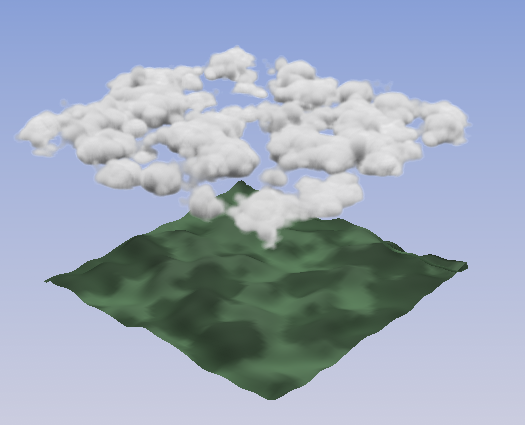
\includegraphics[width=0.7\textwidth]{cloud_impl.png}
	\caption{Визуализация динамической сцены с облаками.}
	\label{fig:cloud-impl}
\end{figure}

На рисунке~\ref{fig:cloud-impl2} представлен результат визуализации динамической сцены с облаками с другого ракурса и с другим положением солнца.
\begin{figure}[htb!]
	\centering
	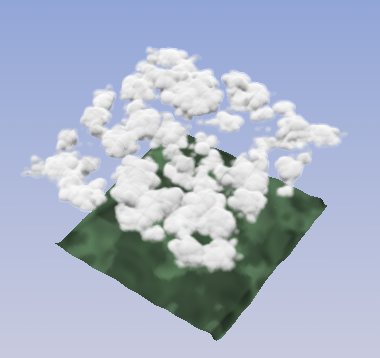
\includegraphics[width=0.65\textwidth]{cloud_impl3.png}
	\caption{Визуализация динамической сцены с облаками с другого ракурса.}
	\label{fig:cloud-impl2}
\end{figure}
\clearpage

На рисунке~\ref{fig:sun-interface} представлен интерфейс управления азимутальным углом солнца.
\begin{figure}[htb!]
	\centering
	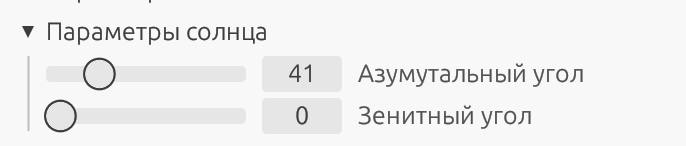
\includegraphics[width=0.65\textwidth]{sun_interface.png}
	\caption{Интерфейс управления азимутальным углом солнца.}
	\label{fig:sun-interface}
\end{figure}

На рисунке~\ref{fig:cloud-interface} представлен интерфейс управления параметрами облаков.
\begin{figure}[htb!]
	\centering
	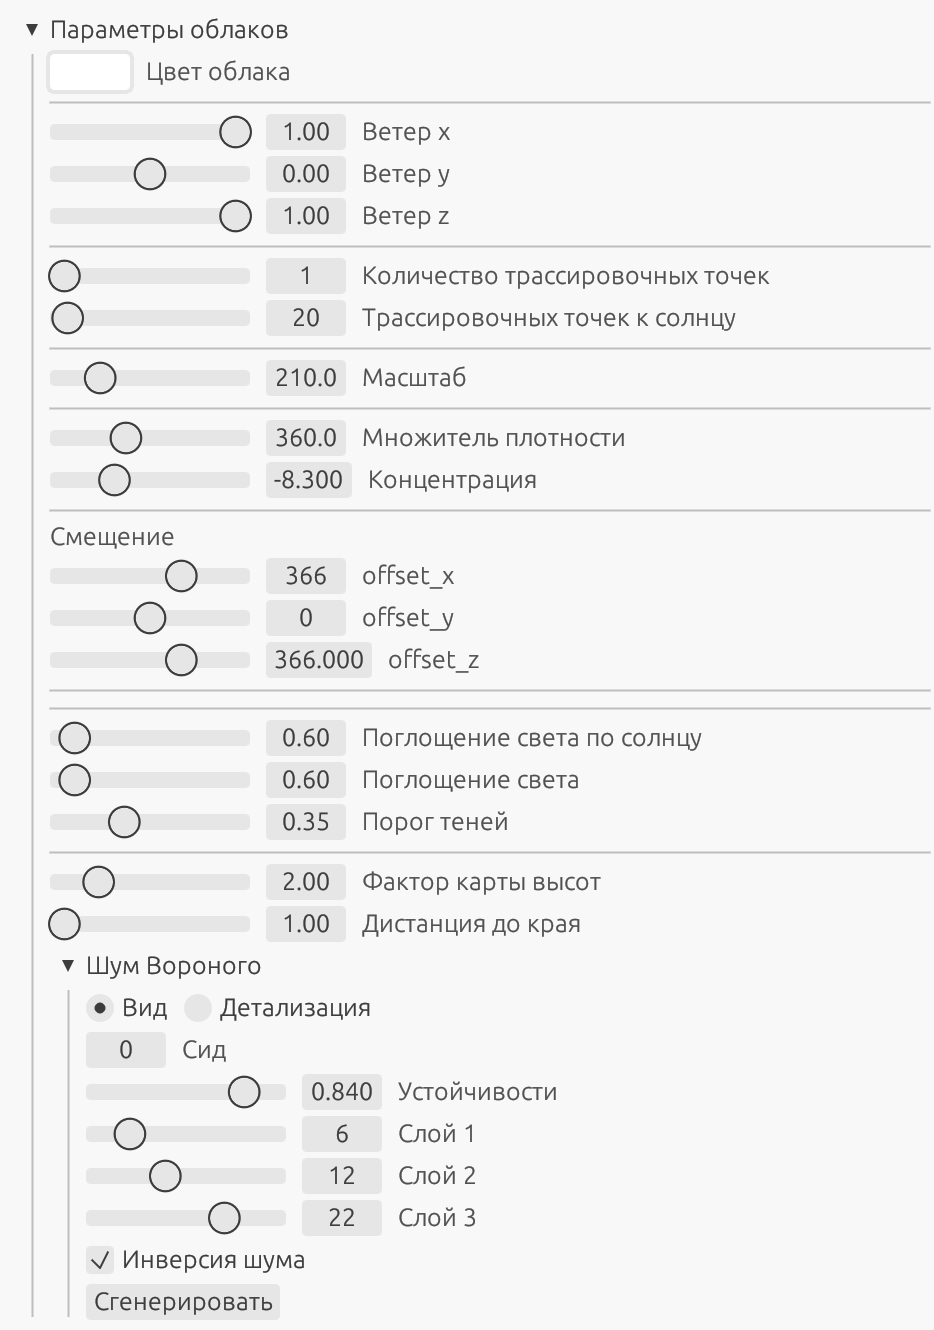
\includegraphics[width=0.65\textwidth]{cloud_interface.png}
	\caption{Интерфейс управления параметрами облаков.}
	\label{fig:cloud-interface}
\end{figure}
\clearpage
На рисунке~\ref{fig:terrain-interface} представлен интерфейс управления параметрами ландшафта.
\begin{figure}[htb!]
	\centering
	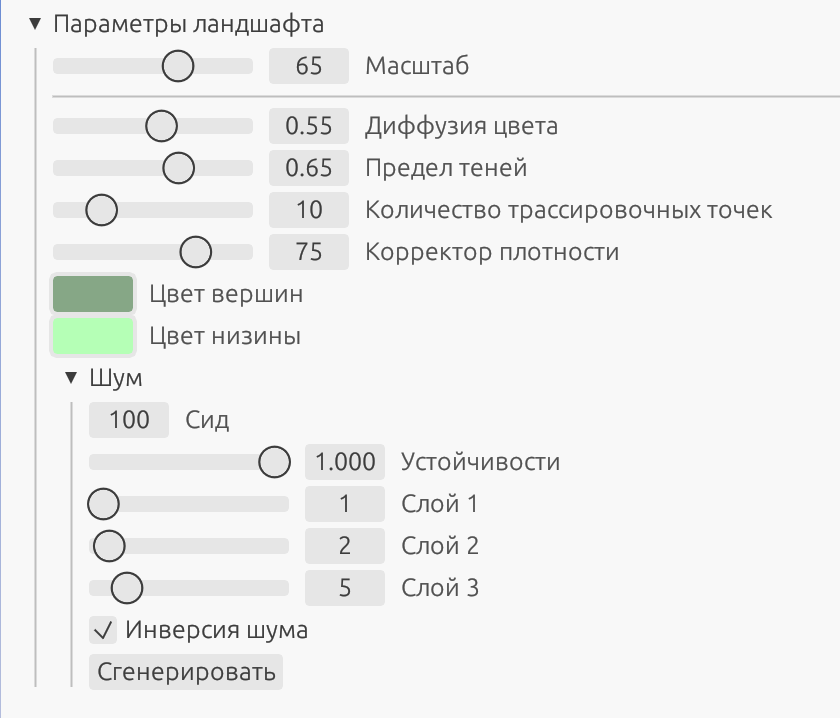
\includegraphics[width=0.65\textwidth]{terrain_interface.png}
	\caption{Интерфейс управления параметрами ландшафта.}
	\label{fig:terrain-interface}
\end{figure}

\section*{Вывод}
В данном разделе был обоснован выбор средств реализации программного обеспечения и представлены детали реализации: реализация алгоритмов и интерфейс программы. Проведено модульное тестирование программы -- тесты пройдены успешно. Также собрана информация о покрытии программы модульными тестами -- 19.83\%.
